\documentclass{beamer}

%French-specific
\usepackage[french]{babel}
\usepackage[autolanguage]{numprint}

%Hyphenation
\usepackage{hyphenat}
\hyphenation{mate-mática recu-perar}

\usetheme{default}
\title{Tamis référentiel}
\author{David Véron}
\date{\today}

\begin{document}

\begin{frame}
    \titlepage
\end{frame}

\begin{frame}{Plan}
    \tableofcontents[hideallsubsections]
\end{frame}

\AtBeginSection[]
{
    \begin{frame}{Plan}
        \tableofcontents[currentsection]
    \end{frame}
}

\section{Bases}

\subsection{Action sûre}
\begin{frame}{Action sûre}
    \begin{block}{Action sûre}
        Un joueur a une \emph{action sûre} s'il sait qu'il peut:
        \begin{itemize}
            \item jouer une carte.
            \item défausser une carte.
        \end{itemize}
    \end{block}
    \begin{block}{Occupé}
        Un joueur ayant une \emph{action sûre} est dit \emph{occupé}.
    \end{block}
    \begin{block}{Verrou}
        L'équipe a des moyens de dire à un joueur qu'il n'a pas d'\emph{action
        sûre}. Ce joueur est dit \emph{verrouillé} il n'a pas le droit de
        défausser tant qu'il n'a pas reçu un nouveau signal pour
        jouer/défausser.
    \end{block}
\end{frame}

\subsection{Défause}
\begin{frame}{Défausse}
    \begin{block}{Défausse}
        Un joueur qui n'a pas reçu d'indice et qui n'a pas d'action sûre a la
        permission de défausser. Dans ce cas il défausse sa carte la plus
        récente n'ayant pas d'indice que nous appellerons \emph{côtelette}.
    \end{block}
\end{frame}

\subsection{Principe du tamis}
\begin{frame}{Principe du tamis}
    \begin{block}{Principe du tamis}
        Si un joueur a un \emph{côtelette} importante, l'équipe peut la sauver
        en fournissant une \emph{action sûre} au joueur.
    \end{block}
\end{frame}

\subsection{Déchet}
\begin{frame}{Déchet}
    \begin{block}{Déchet}
        Autre copie d'une carte déjà jouée ou qui a reçu un indice pour être
        jouée.
    \end{block}
\end{frame}

\subsection{Principe de bon touché}
\begin{frame}{Principe de bon touché}
    \begin{block}{Principe de bon touché}
        Un joueur qui ne sait pas si une carte sur laquelle il vient de
        recevoir un indice est un déchet doit partir du principe que ce n'en
        est pas un.
    \end{block}
    \begin{block}{Toucher}
        Une carte est toucée par un indice si elle passe de l'état sans indice
        à l'état avec indice par ce dernier.
    \end{block}
\end{frame}

\subsection{Seuil}
\begin{frame}{Seuil}
    \begin{block}{Seuil}
        Le seuil est le plus petit rang qu'il reste à jouer. Par exemple\ : 2.
        \begin{figure}[h]
            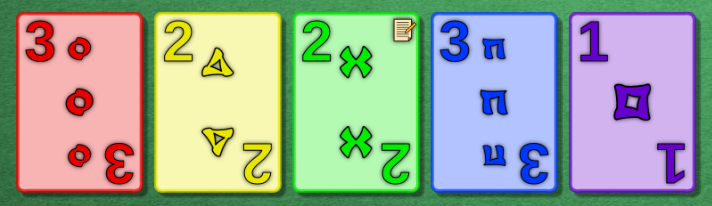
\includegraphics[width=\textwidth]{threshold.png}
        \end{figure}
    \end{block}
\end{frame}

\subsection{Indice référentiel}
\begin{frame}{Indice référentiel}
    \begin{block}{Indice référentiel}
        Un indice référentiel donne une indication pour jouer/défausser une
        carte par rapport aux cartes qui viennent de recevoir un indice.

        Chaque indice référentiel a un \emph{centre} et une \emph{cible}.
    \end{block}
    \begin{block}{Centre}
        Le centre d'un indice référentiel est la carte la plus récente qui
        vient d'être touchée.
    \end{block}
    \begin{block}{Cible}
        La cible est la carte à jouer/défausser d'un indice référentiel. Sa
        position se déduit par rapport au centre.
    \end{block}
\end{frame}

\section{Indice}

\subsection{Indice de jeu direct}
\begin{frame}{Indice de jeu direct}
    \begin{block}{Indice de jeu direct}
        Cible := centre ie joue la carte touchée la plus récente.
    \end{block}
\end{frame}

\subsection{Indice de rang}
\begin{frame}{Indice de rang}
    \begin{figure}[h]
        \includegraphics[width=\textwidth]{rank.png}
    \end{figure}
\end{frame}

\subsection{Indice de couleur}
\begin{frame}{Indice de couleur}
    \begin{block}{Indice de couleur}
        Bientôt des indices de jeu référentiels. Pour l'instant un indice de
        jeu direct.
    \end{block}
\end{frame}

\subsection{Indice de recoupage}
\begin{frame}{Indice de recoupage}
    \begin{block}{Indice de recoupage}
        Si une carte a déjà un indice et un second indice révèle entièrement
        son identié la rendant jouable/défaussable. L'indice n'a rien de
        référentiel et n'a pour but que de faire jouer/défausser la dite
        carte.
    \end{block}
\end{frame}

\subsection{Indice de défausse référentiel}
\begin{frame}{Indice de défausse référentiel}
    \begin{block}{Indice de défausse référentiel}
        La cible, la carte à défausser est la carte non-touchée précédent le
        centre.
    \end{block}
    \begin{block}{Verrouillage}
        Un indice de défausse référentiel qui s'enroule autour de la main et
        revient sur la côtelette, verrouille ce joueur.
    \end{block}
\end{frame}

\begin{frame}{Exemple - 1}
    Le seuil est à 1.
    \begin{figure}[h]
        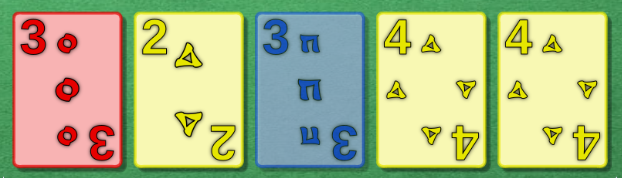
\includegraphics[width=0.7\textwidth]{ref_discard_before.png}
    \end{figure}
    Indice 2.
    \begin{figure}[h]
        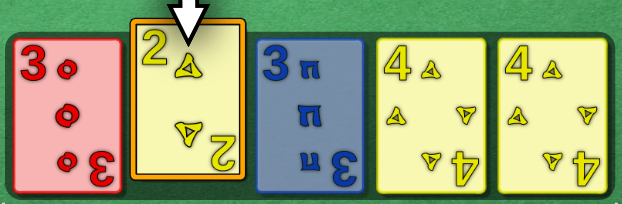
\includegraphics[width=0.7\textwidth]{ref_discard_after.png}
    \end{figure}
    Défausse le 3 bleu.
\end{frame}

\begin{frame}{Exemple - 2}
    Le seuil est à 2.
    \begin{figure}[h]
        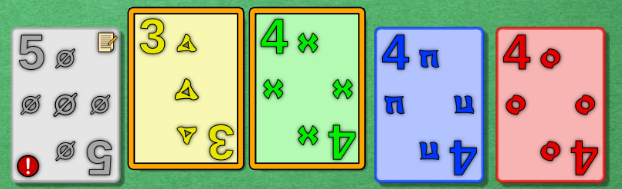
\includegraphics[width=0.5\textwidth]{lock_before.png}
    \end{figure}
    Indice 4.
    \begin{figure}[h]
        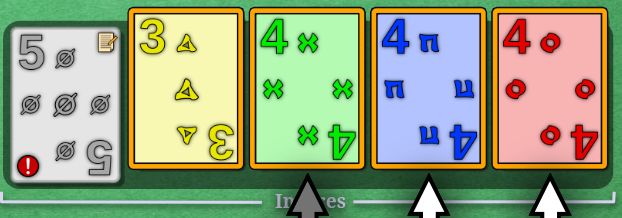
\includegraphics[width=0.5\textwidth]{lock_after.png}
    \end{figure}
    \begin{itemize}
    \item 4 vert n'est ni jouable ni défaussable.
        \begin{itemize}
            \item Ce n'est pas un recoupage.
            \item C'est un indice de défausse référentiel.
        \end{itemize}
        \item Le \emph{centre} est le 4 bleu. La \emph{cible} est le 5 null qui
              est aussi la \emph{côtelette}, l'indice est donc un verrouillage.
    \end{itemize}
\end{frame}

%\subsection{Indice de jeu référentiel}

%\section{Avancé}

%\subsection{Incitation}

%\subsection{Impasse}

\end{document}
